% 32-11(32쪽) — $y=4^{x+a}+b$ 의 그래프(원문 「오른쪽 그림」). 스캔 화질이 낮아 TikZ 로 다시 그림.
% 라벨은 원문에 있는 것만 둔다 — $y$절편 $2$, 점근선 자리의 $-2$(점선), $\pt{O}$, 곡선 이름 $y=4^{x+a}+b$.
% $a$, $b$ 의 값(답)은 그림에서 읽히지 않게 적지 않는다.
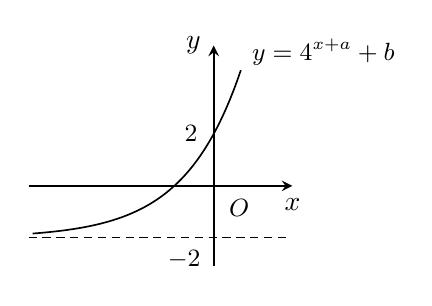
\begin{tikzpicture}[line width=0.6pt, x=1.0cm, y=0.33cm, >=stealth]
  \draw[densely dashed, line width=0.4pt] (-2.35,-2) -- (0.95,-2);
  \draw[->, line width=0.7pt] (-2.35,0) -- (1.00,0) node[below=1pt] {$x$};
  \draw[->, line width=0.7pt] (0,-3.1) -- (0,5.4) node[left=1pt] {$y$};
  \draw[domain=-2.30:0.345, samples=80, smooth] plot (\x, {pow(4,\x+1)-2});
  \node[anchor=east, font=\small] at (-0.08,2) {$2$};
  \node[anchor=north east, font=\small] at (-0.04,-2.1) {$-2$};
  \node[anchor=north west, font=\small] at (0.07,-0.15) {$\pt{O}$};
  \node[anchor=south west, font=\small] at (0.36,4.25) {$y=4^{x+a}+b$};
\end{tikzpicture}
